\chapter{相关数学知识}
本附录列出了部分有关的数学知识。这些知识并非必要的内容,但掌握它们可以让你对C++语言有更深入的理解。
\section{数制转换}
\subsection*{简介与概念引入}
图C.1是一个数字时钟的界面,它指示的日期是2016年08月29日,时间是20:34:42。\par
\begin{figure}[htbp]
    \centering
    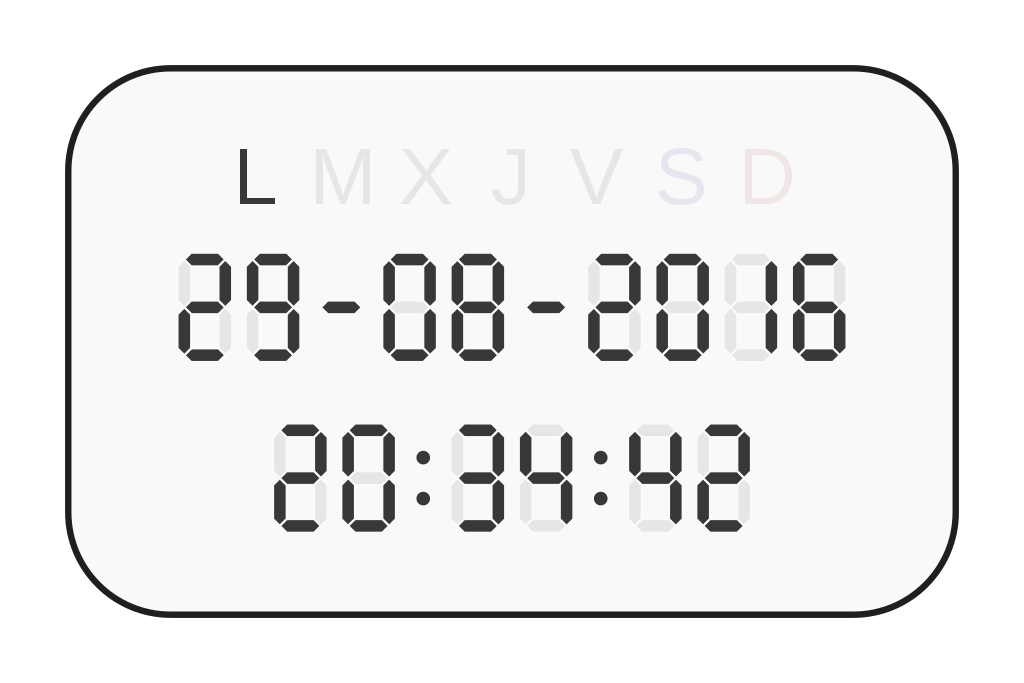
\includegraphics[width=0.5\textwidth]{../images/other_parts/C_digital_clock.png}
    \caption{一个简单的数字时钟}
    \footnotesize{图片来源:维基共享资源}
\end{figure}
每一秒,这个数字时钟显示的时间都会发生变化,变化主要体现在``秒''这一位上。我们很容易就能想象出来,下一步它会变成43,再下一秒它会变成44,就这样每一秒都增加1,直到59——这是一个例外,下一步它不是变成60,而是变成了00。同时发生变化的还有``分''这一位,它会变成35。\par
如果``分''位不发生变化,我们会在20:34:59的下一秒看到20:34:00。这会给我们造成一种错觉,好像我们回到了60秒之前。但是``分''位发生了变化,这就很明确地告诉我们,现在是20:35:00,刚才是20:34:00,这俩不一样。\par
此后的每一分钟都是如此。每当``秒''走到59的时候,下一步它就会变成00,同时``分''增加1,直到``分''也遇到了59,这时它再加就有困难了,因为``分''这一位没有60,所以它只能变回00,同时让``时''增加1。这就是一个\textbf{进位(Carry)}过程。\par
为什么要进位?这是因为,只用一位数字能表示的范围太小,一旦我们进行计数,就很容易出现不够的情况。比如说时钟,如果它只``秒''位,那么它就会每60秒一循环,从00加到59又变成了00\footnote{这是一种溢出(Overflow)现象。},这怎么合理呢?\footnote{一个现实的例子就是干支纪年法。天干地支轮相更替,60年作一循环,但它没有进位机制,只有一个干支位,所以我们不能单纯根据一个``丙申''判断它是1176年还是2016年还是别的年份,必须依赖其它信息作为参考。}但是加上了``分''这一位之后,我们只需要在每次``秒''超过59不能再加的时候,把``秒''变回00,并且在``分''位上进位,就可以正确记录它的变化了。\textbf{所以我们可以说,秒是``逢60进一''的。}\par
仅仅有``分''位还是不够,它也有60分钟一循环的问题,所以我们还有``时''。每当分超过了59不能再加的时候,就可以把``分''变回00,并且在``时''位上进位,这样又可以正确记录它的变化了。所以说,分也是``逢60进一''的。\par
同样的道理,我们可以看出,时是``逢24进一''的。至于``日'',它的进位规则就比较麻烦了,本书就不再细究。\par
我们在日常生活中最常用的是10进制。对于``个位''来说,它只能表示从0到9的10种情况。在计数的时候,一旦超过了9,我们就需要进位:让``十位''加1\footnote{原来的十位是0,我们省略不写。},同时个位变回0。所以说,个位是``逢10进一''的。\par
两位数只能表示100种情况,我们依然可能遇到不够的情况。当我们加到超过99的时候,就需要再进位了。这个进位过程可以分为两步:
\begin{enumerate}
    \item 个位进位。进位之后个位变为0,而十位加1,变为``9+1''。我们发现,这个值超过了十位能表示的范围,所以十位也需要进位。
    \item 十位进位。进位之后十位变为0,而百位加1,变为1。至此进位完成。
\end{enumerate}
当我们熟悉了整个过程之后,我们就根本不用分成两步来进位了,直接下意识得到99+1=100就行。总之,十位也是``逢10进一''的。\par
一个十进制整数的每一位都满足这样``逢10进一''的规则,所以我们对每一位都可以仿照此理来进行推导。于是我们把计数推广到加法(加法就是重复若干次的计数过程),再把加法推广到乘法(若干次同样的加法过程),再把乘法推广到乘方(若干次同样的乘法过程),乃至高德纳箭头\footnote{高德纳箭头(Knuth's up-arrow notation),由高德纳在1976年提出,它是一种表示巨大整数的方法,可以视作是对重复乘方的迭代扩展。}。图C.2展示了这样一个过程,我们就是从这里开始学习数学的。\par
\begin{figure}[htbp]
    \centering
    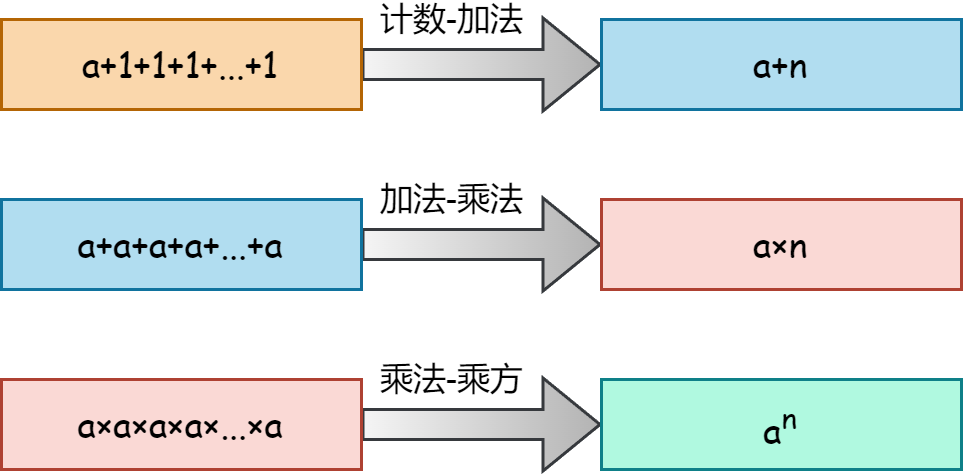
\includegraphics[width=0.75\textwidth]{../images/other_parts/C_from_counting_to_exponentiation_300.png}
    \caption{从计数到乘方}
\end{figure}
我们在小学时都背过加法表和乘法表,它就是10进制整数的计算规则。但是如果换一套进制呢,情况就会发生变化了。图C.3就是一个12进制乘法表,仅供读者开拓眼界。\par
\begin{figure}[htbp]
    \centering
    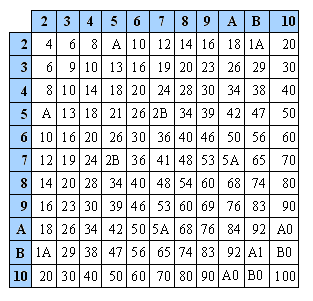
\includegraphics[width=0.5\textwidth]{../images/other_parts/C_duodecimal_multiplication_table.png}
    \caption{一个12进制乘法表}
    \footnotesize{图片来源:维基共享资源}
\end{figure}
\subsection*{数的形式化表示}
有这样一个十进制的三位数,它的百位是$a$,十位是$b$,个位是$c$,怎么把这个数表示出来呢?我们可以用$100a+10b+c$的形式来表示。\par
同样的道理,如果我们知道了某个整数的每一位,那我们就可以用每一位乘$10^n$再求和的形式把它表示出来。
\begin{align*}
36={}&3\times10^1+6\times10^0\\
1024={}&1\times10^3+0\times10^2+2\times10^1+4\times10^0\\
32768={}&3\times10^4+2\times10^3+7\times10^2+6\times10^1+8\times10^0
\end{align*}
所以我们可以把它抽象一下:对于任意一个整数$a$,它可以用它的每一位$a_n$乘以$10^n$求和表示成
\begin{align*}
a=a_0\times10^0+a_1\times10^1+a_2\times10^2+\ldots+a_n\times10^n+\ldots
\end{align*}
其中$a_0$是个位,$a_1$是十位,$a_2$是百位,以此类推。我们还可以用求和符号简写成这样:
\begin{align*}
a=\sum_{n=0}^{+\infty}a_n10^n
\end{align*}\par
如果要表示一个小数呢?我们就需要把$n$扩展到负数范围中来。
\begin{align*}
3.14159={}&3\times10^0+1\times10^{-1}+4\times10^{-2}+1\times10^{-3}+5\times10^{-4}+9\times10^{-5}\\
0.5772={}&0\times10^0+5\times10^{-1}+7\times10^{-2}+7\times10^{-2}+2\times10^{-3}
\end{align*}
所以我们还可以把这个数写成这样:
\begin{align*}
a=\ldots+a_2\times10^2+a_1\times10^1+a_0\times10^0+a_{-1}\times10^{-1}+a_{-2}\times10^{-2}+\ldots
\end{align*}
其中的$a_{-1}$是十分位,$a_{-2}$是百分位,$a_{-3}$是千分位,以此类推。我们还可以用求和符号简写成这样:
\begin{align*}
a=\sum_{n=-\infty}^{+\infty}a_n10^n
\end{align*}\par
以上全都是基于十进制来讨论的。如果换一个进制呢?我们只需要把$10$改换成对应的数就可以了。这是二进制:
\begin{align*}
a=\sum_{n=-\infty}^{+\infty}a_n2^n
\end{align*}
这是八进制:
\begin{align*}
a=\sum_{n=-\infty}^{+\infty}a_n8^n
\end{align*}
这是十六进制\footnote{在十六进制中,用一位阿拉伯数字不足以表示一位数,所以引入$a$(也可大写)表示$10$,$b$表示$11$,$c$表示$12$,$d$表示$13$,$e$表示$14$,$f$表示$15$。}:
\begin{align*}
a=\sum_{n=-\infty}^{+\infty}a_n16^n
\end{align*}\par
假如我们有一个十进制\footnote{为了把不同进制下的数字区分开,我们在数字之外套上括号并用下标注明是何种进制。}的$a=(1024)_{10}$和一个十六进制的$b=(400)_{16}$,如何判断它们是否相等呢?很简单,我们只需要验证
\begin{align*}
\sum_{n=-\infty}^{+\infty}a_n10^n=\sum_{m=-\infty}^{+\infty}b_n16^n
\end{align*}
就可以了。等号左边是$1\times10^3+2\times10^1+4\times10^0=1024$,\footnote{对于十进制数,可以不用这么麻烦,直接1024就行。}而右边是$4\times16^2=1024$,所以等号成立,$(1024)_{10}=(400)_{16}$就是相等的。\par
而$(153)_8$和$(211)_7$不相等,这是因为
\begin{align*}
(153)_8={}&1\times8^2+5\times8^1+3\times8^0=107\\
(211)_7={}&2\times7^2+1\times7^1+1\times7^0=106
\end{align*}
这里的$107$和$106$不相等。\par
所以说$(a)_R=\sum_{n=-\infty}^{+\infty}a_nR^n$就是我们对$(a)_R$这个数的形式化表示。只要知道这个数的每一位,我们就能确定这个数的值。\par
不过这么写还是有一点麻烦,所以我们还可以自行搞一套符号来简化$\sum_{n=-\infty}^{+\infty}a_nR^n$,我们可以写成这样:
\begin{align*}
(a)_R=\sum_{n=-\infty}^{+\infty}a_nR^n=\left[\ldots,a_2,a_1,a_0;a_{-1},a_{-2},\ldots\right]_R
\end{align*}
其中的分号用来分隔个位与十分位。举几个例子:
\begin{align*}
(10)_{10}={}&\left[1,0;\right]_{10}\\
(1010)_2={}&\left[1,0,1,0;\right]_2\\
(0.75)_{10}={}&\left[0;7,5\right]_{10}\\
(0.c)_{16}={}&\left[0;12\right]_{16}\\
(1a.c3)_{16}={}&\left[1,10;12,3\right]_{16}
\end{align*}
这里的$(10)_{10}$与$(1010)_2$是相等的,$(0.75)_{10}$与$(0.c)_{16}$也是相等的,读者可以自行计算验证。\footnote{我们把$\;]$内的数字都用十进制来表示,这样会方便我们计算。毕竟我们还是最熟悉十进制。}而$(1a.c3)_{16}$的表示可以参考图C.4来理解。\par
\begin{figure}[htbp]
    \centering
    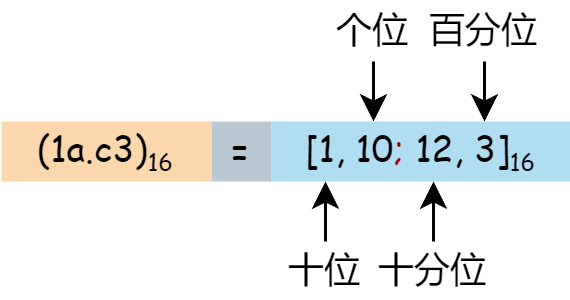
\includegraphics[width=0.6\textwidth]{../images/other_parts/C_formatted_representation_of_a_number_300.png}
    \caption{$(1a.c3)_{16}$的形式化表示}
\end{figure}
\subsection*{进位与借位}
现在让我们用形式化的表示方法来计算一下$(c)_{16}+(f)_{16}$的值。
\begin{align*}
(c)_{16}={}&[12;]_{16}\\
(f)_{16}={}&[15;]_{16}\\
[12;]_{16}+[15;]_{16}={}&[27;]_{16}
\end{align*}
现在我们得到了一个数,它的个位是$27$,这已经超过十六进制的最大限制$15$了,那么我们怎么办?当然是\textbf{进位}了。
\begin{align*}
[27;]_{16}=[1,27-16;]_{16}=[1,11;]_{16}=(1b)_{16}
\end{align*}
我们怎么判断这个结果是不是正确呢?很简单,用十进制的计算结果$(27)_{10}$和$(ab)_{16}$比较一下就好了,也就是验证
\begin{align*}
\sum_{n=-\infty}^{+\infty}a_n10^n=\sum_{n=-\infty}^{+\infty}b_n16^n
\end{align*}
最后我们会发现$1\times16^1+11\times16^0=27$确实成立,所以计算结果无误。\par
这里的进位过程非常简单,就是``后一位减16,同时前一位加1''。如果换到十进制下,那就是``后一位减10,同时前一位加1''。
\begin{align*}
[9,9,10;]_{10}=[9,10,0;]_{10}=[10,0,0;]_{10}=[1,0,0,0;]_{10}
\end{align*}
所以说同样是$(1000)_{10}$这个数字,我们写成$[1,0,0,0;]_{10}$和$[9,9,10;]_{10}$,甚至写成$[9,9,9;9,9,10]_{10}$都是对的。正确的写法有无数种,但最简单的写法还是进位之后的写法。\par
而在计算过程当中,我们没那么多限制,可以任意选择自己喜欢的写法。比如说,我们做减法运算时,就可能涉及到\textbf{借位(Borrow)}操作。这就是在不同形式之间进行变化,从而简化计算的方法。\par
举个例子,我们要计算$(12.6)_8-(7.7)_8$,这时我们就可以通过把$[1,0;6]_8$转换成我们方便计算的形式。注意它是八进制的,所以借位的规则是``后一位加8,同时前一位减1''。
\begin{align*}
{}&[1,2;6]_8-[7;7]_8\\
={}&[10;6]_8-[7;7]_8\\
={}&[9;14]_8-[7;7]_8\\
={}&[2;7]_8
\end{align*}
所以$(12.6)_8-(7.7)_8=(2.7)_8$。\par
以上是进1的情况,实际计算时我们可能进2,进3或者进4,例如$[56,111;54]_{10}$。这种情况下我们最好用带余除法来进位。先看十分位:\par
\begin{align*}
54\div10=5\ldots4
\end{align*}
所以我们进5,也就是十分位减$5\times10=50$,同时个位加$5$,变成$[56,116;4]_{10}$。再看个位:
\begin{align*}
116\div10=11\ldots6
\end{align*}
所以我们进11,也就是个位减$11\times10=110$,同时十位加$11$,变成$[67,6;4]_{10}$。再看十位:
\begin{align*}
67\div10=6\ldots7
\end{align*}
所以我们进6,也就是十位减$6\times10=60$,同时百位加$6$,变成$[6,7,6;4]_{10}$,这样整理完了就会得到$(676.4)_{10}$。\par
换一个$R$进制,思路也不变,我们只需要把除数从$10$改成$R$就行了。所以$[0;500]_{16}$就可以这样处理:
\begin{align*}
{}&[0;500]_{16}\\
500\div16=31\ldots4\;\Rightarrow\;{}&[31;4]_{16}\\
31\div16=1\ldots15\;\Rightarrow\;{}&[1,15;4]_{16}
\end{align*}
最后把$[1,15;4]_{16}$写成十六进制数的形式$(1f.4)_{16}$就可以了。\par
\subsection*{数制转换的一般方法}
接下来我们考虑如何进行数制转换。假如我们有一个$R$进制的数$a$,希望转换成$T$进制的数$x$,那么只需要找到一个$[\ldots,x_2,x_1,x_0;x_{-1},x_{-2},\ldots]$,能满足式子
\begin{align*}
\sum_{n=-\infty}^{+\infty}a_nR^n=\sum_{m=-\infty}^{+\infty}x_nT^n
\end{align*}
就可以了。\par
在这里,我们把$a$拆成整数部分和小数部分来考虑。对于整数部分,我们用到的思路和进位相似;而对于小数部分,我们用到的思路和借位相似。在分别处理完整数和小数的转换之后,我们只需把结果相加即可。\par
\subsubsection*{整数部分}
如果某个$R$进制整数要转换成十进制,那就非常简单,直接用$\sum_{n=0}^{+\infty}a_nR^n$算出来就行。以下是例子:
\begin{align*}
&(4d9)_{16}=4\times16^2+13\times16^1+9\times16^0=(1241)_{10}\\
&(1001011)_2=1\times2^6+1\times2^3+1\times2^1+1\times2^0=(75)_{10}\\
&(64)_8=6\times8^1+4\times8^0=(52)_{10}
\end{align*}\par
如果要把某个十进制整数转换成$R$进制,我们就可以先把它放在$x$的个位上,然后用$R$进制进位的方式来处理它。例如,要把$(382)_{10}$转换成十六进制,步骤如下:
\begin{align*}
{}&[382;]_{16}\\
382\div16=23\ldots14\;\Rightarrow\;{}&[23,14;]_{16}\\
23\div16=1\ldots7\;\Rightarrow\;{}&[1,7,14;]_{16}\\
1\div16=0\ldots1\;\Rightarrow\;{}&[1,7,14;]_{16}
\end{align*}
最后把$[1,7,14;]_{16}$表达成十六进制的形式$(17e)_{16}$即可。\par
要把$(395)_{10}$转换成八进制,步骤如下:
\begin{align*}
{}&[395;]_8\\
395\div8=49\ldots3\;\Rightarrow\;{}&[49,3;]_8\\
49\div8=6\ldots1\;\Rightarrow\;{}&[6,1,3;]_8\\
6\div8=0\ldots6\;\Rightarrow\;{}&[6,1,3;]_8
\end{align*}
最后把$[6,1,3;]_8$表达成八进制的形式$(613)_8$即可。\par
要把$(41)_{10}$转换成二进制,步骤如下:
\begin{align*}
{}&[41;]_2\\
41\div2=20\ldots1\;\Rightarrow\;{}&[20,1;]_2\\
20\div2=10\ldots0\;\Rightarrow\;{}&[10,0,1;]_2\\
10\div2=5\ldots0\;\Rightarrow\;{}&[5,0,0,1;]_2\\
5\div2=2\ldots1\;\Rightarrow\;{}&[2,1,0,0,1;]_2\\
2\div2=1\ldots0\;\Rightarrow\;{}&[1,0,1,0,0,1;]_2\\
1\div2=0\ldots1\;\Rightarrow\;{}&[1,0,1,0,0,1;]_2
\end{align*}
最后把$[1,0,1,0,0,1;]_2$表达成二进制的形式$(101001)_2$即可。\par
我们不难发现,整个过程的关键其实就是反复对着上一步的商值除以$R$,然后把每一步的余数按照个位、十位、百位的顺序排起来。实际操作中,我们更倾向于用短除法来进行转换,如图C.5所示。\par
\begin{figure}[htbp]
    \centering
    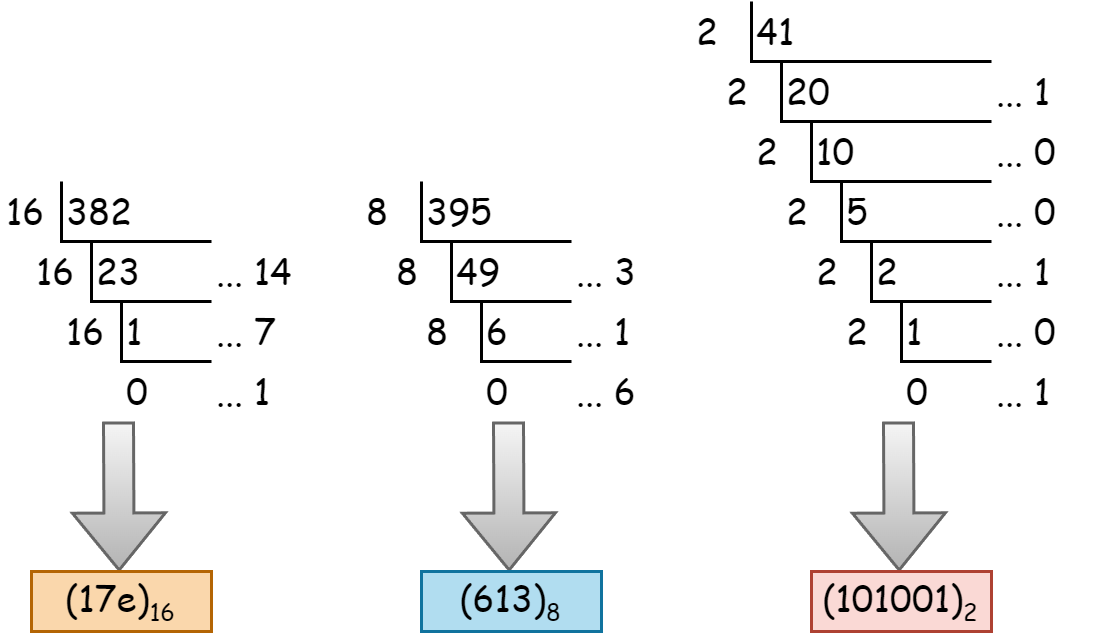
\includegraphics[width=0.75\textwidth]{../images/other_parts/C_short_division_300.png}
    \caption{通过短除法把十进制数转换成$R$进制}
\end{figure}
使用短除法时只需注意,先算出来的余数在个位,后算出来的在十位,以此类推,从低到高。\par
当我们需要把$R$进制数转换成$T$进制时,又该如何做呢?一般我们使用十进制作为中介\footnote{但当我们进行二进制、八进制和十六进制之间的互相转换时,有更简单的方法。详见后文。},先把$R$进制转换为十进制,再把它转换为$T$进制。这样的好处是,我们所有的过程计算都可以基于十进制,尤其是乘和除。如果不用十进制作为中介,那么我们在转换时就需要背$R$进制的乘法表了。\par
\subsubsection*{小数部分}
接下来我们考虑小数部分。\par
如果某个$R$进制小数要转换成十进制,那就非常简单,直接用$\sum_{n=-\infty}^{-1}a_nR^n$算出来就行。以下是例子:
\begin{align*}
{}&(0.1011)_2=1\times2^{-1}+1\times2^{-3}+1\times2^{-4}=0.6875\\    
{}&(0.c8)_{16}=12\times16^{-1}+8\times16^{-2}=0.78125\\
{}&(0.5)_8=5\times8^{-1}=0.625
\end{align*}\par
如果要把某个十进制整数转换成$R$进制,我们就需要用借位的方法来处理它了。我们还是先把它放在个位上,然后用$R$进制借位的方式来处理它。例如,要把$0.78125$转换成十六进制,我们就先写成$[0.78125;]_{16}$。\par
怎么借位呢?试想,如果我们要从前一位借1,那么就要向后一位加16;如果我们要从前一位借2,那么就要向后一位加32,……。那么我们现在想从前一位借$0.78125$呢?自然是把它乘上16加到后一位中了。
\begin{align*}
0.78125\times16=12.5\;\Rightarrow\;[0;12.5]_{16}
\end{align*}
接下来我们发现十分位上还有小数,那么我们就借$0.5$,把它乘上16加到后一位去——只有这样才能把十分位变成整数。
\begin{align*}
0.5\times16=8\;\Rightarrow\;[0;12,8]_{16}
\end{align*}
这样就完成了。最后只需要把它整理成$(0.c8)_{16}$即可。\par
再举一个例子,把$(0.669)_{10}$转换成二进制的操作是
\begin{align*}
{}&[0.669;]_2\\
0.669\times2=1.338\;\Rightarrow\;{}&[0;1.338]_2\\
0.338\times2=0.676\;\Rightarrow\;{}&[0;1,0.676]_2\\
0.676\times2=1.352\;\Rightarrow\;{}&[0;1,0,1.352]_2\\
0.352\times2=0.704\;\Rightarrow\;{}&[0;1,0,1,0.754]_2\\
\ldots\;\ldots{}&
\end{align*}
小数的进制转换是有可能算不尽的,所以我们根据实际的精度需要来近似就行。这个数的二进制结果在$(0.1010)_2$到$(0.1011)_2$之间,我们可以取$(0.101)_2$作为近似。\par
再举一例,把$(0.35)_{10}$转换成八进制的步骤可以这样:
\begin{align*}
{}&[0.35;]_8\\
0.35\times8=2.8\;\Rightarrow\;{}&[0;2.8]_8\\
0.8\times8=6.4\;\Rightarrow\;{}&[0;2,6.4]_8\\
0.4\times8=3.2\;\Rightarrow\;{}&[0;2,6,3.2]_8\\
0.2\times8=1.6\;\Rightarrow\;{}&[0;2,6,3,1.6]_8
\end{align*}\par
总而言之,就是把整数部分作为这一位,而把小数部分乘以$R$加到下一位,这样``借位''。\par
至于$R$进制转$T$进制,思路还是以十进制作为桥梁,先转成十进制,再转成$T$进制。\par
\subsection*{二、八、十六进制间的特殊转换方法}
前文介绍的一般方法,已经可以用于在二进制、八进制和十六进制数之间进行转换。但对于它们三者之间的转换来说,用十进制作为桥梁还是太麻烦了一点。在这里,我们有更好的方案。\par
以二进制数$a$转换成八进制数$x$为例,我们可以进行如下数学推导(看不懂请跳过):
\begin{align*}
\sum_{n=-\infty}^{+\infty}a_n2^n=\sum_{m=-\infty}^{+\infty}(a_{3m+2}2^2+a_{3m+1}2^1+a_{3m}2^0)8^m=\sum_{m=-\infty}^{+\infty}x_m8^m
\end{align*}
所以只要
\begin{align*}
x_m=a_{3m+2}2^2+a_{3m+1}2^1+a_{3m}2^0
\end{align*}
就可以保证这个转换是正确的。\par
具体来说,如何操作呢?我们可以在分号左右两边,每三位一组(如果不到三个数字,不妨在两侧补0),把它转换成八进制。以$(10101.1101)_2$为例,我们把$[1,0,1,0,1;1,1,0,1]_2$以分号为界,向左向右每三位一组,转换成八进制,这就是图C.6中从上到下的过程。\par
\begin{figure}[htbp]
    \centering
    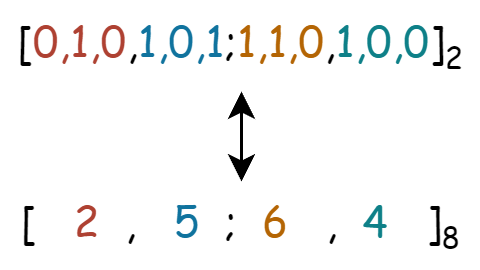
\includegraphics[width=0.5\textwidth]{../images/other_parts/C_bin_to_oct_300.png}
    \caption{二进制与八进制的转换}
\end{figure}
那么拿到$(25.64)_8$之后我们也可以反过来,把每一位转换成三位一组的二进制形式,也就是图C.6中从下到上的过程。\par
十六进制也是同理,
\begin{align*}
\sum_{n=-\infty}^{+\infty}a_n2^n=\sum_{m=-\infty}^{+\infty}(a_{4m+3}2^3+a_{4m+2}2^2+a_{4m+1}2^1+a_{4m}2^0)16^m=\sum_{m=-\infty}^{+\infty}x_m8^m
\end{align*}
所以只要
\begin{align*}
x_m=a_{4m+3}2^3+a_{4m+2}2^2+a_{4m+1}2^1+a_{4m}2^0
\end{align*}
就可以保证这个转换是正确的。\par
具体操作和二进制转八进制相似,只是三位一组变成了四位一组。还以$(10101.1101)_2$为例,我们把$[1,0,1,0,1;1,1,0,1]_2$以分号为界,向左向右每四位一组(如果不到四个数字,不妨在两侧补0),转换成十六进制,这就是图C.7中从上到下的过程。\par
\begin{figure}[htbp]
    \centering
    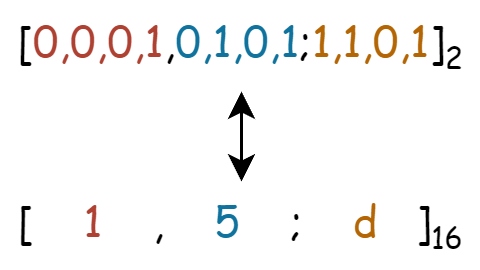
\includegraphics[width=0.5\textwidth]{../images/other_parts/C_bin_to_hex_300.png}
    \caption{二进制与十六进制的转换}
\end{figure}
那么拿到$(15.d)_{16}$之后我们也可以反过来,把每一位转换成四位一组的二进制形式,也就是图C.7中从下到上的过程。\par
如果要在八进制与十六进制之间进行转换,最简单的方式是以二进制为桥梁,先把$(15.d)_{16}$转换成$(10101.1101)_2$,再转换成$(25.64)_8$。\par
